\documentclass[a4paper]{article}

\usepackage[utf8]{inputenc}
\usepackage[T1]{fontenc}
\usepackage{textcomp}
\usepackage[italian]{babel}
\usepackage{amsmath, amssymb}
\usepackage{listings}
\usepackage{graphicx}
\usepackage{hyperref}
\usepackage{siunitx}

\title{Relazione di Laboratorio 1 - Pendolo Fisico}
\author{Walhout Francesco - Iallorenzi Michele}

\begin{document}
    \maketitle
    
    \section{Introduzione}
    Il Pendolo Fisico, anche chiamato Pendolo Composto, è un pendolo che, a differenza del classico pendolo con una massa e filo ideale (inestensibile e privo di massa) attaccato al punto di sospensione, ha una massa del filo non trascurabile. Si può chiamare pendolo fisico un qualsiasi oggetto, attaccato ad un punto di sospensione, libero di oscillare. Esempi più classici di pendoli fisici sono delle aste di un materiale con densità costante. Nel nostro caso avremo un'asta metallica forata, che oscilla su uno dei fori (punti di sospensione). Lo scopo dell'esperimento è quello di misurare i periodi di oscillazione del pendolo, in funzione della distanza tra centro di massa e punto di sospensione, e confrontare i dati con un modello matematico, verificando che questo descriva al meglio il fenomeno fisico grazie ad un fit dei minimi quadrati.
    
    \section{Esperienza}
    
    \subsection{Strumenti}
    \begin{itemize}
        \item Un'asta metallica forata.
        \item Un supporto di sospensione.
        \item Cronometro (risoluzione $\SI{0.01}{\s}$)
        \item Metro a nastro (risoluzione $\SI{1}{\mm}$)
        \item Calibro ventesimale (risoluzione $\SI{0.05}{\mm}$)
    \end{itemize}
    
    \subsection{Misurazione}
    L'esperimento prevede di misurare la durata totale di 10 oscillazioni per 5 volte, per un totale di 50 oscillazzioni;
    abbiamo utilizzato come misura la media di questi 5 tempi, che è stata divisa per $10$ per ottenere la durata
    di una singola oscillazzione, col vantaggio di ridurre di $10$ volte l'incertezza di misura.
    Il procedimento è stato ripetuto 10 volte, per ciascuno dei punti di sospensione.\\
    Per misurare un oscillazione completa, partendo da una certa ampiezza iniziale del pendolo, è necessario contare gli istanti in cui il pendolo si ferma completamente, quindi assicurandosi che le oscillazioni siano complete.
    Dato che abbiamo azionato manualmente il cronometro osservando il pendolo, abbiamo
    utilizzato come incertezza di misura il tempo di reazione umano medio, ovvero $\SI{0.2}{\s}$,
    che per l'accorgimento descritto precedentemente verrà diviso per $10$.\\
    La tabella \ref{tab:dati} mostra, per ciascun punto di sospensione, le $5$ misure,
    ciascuna di  $10$ periodi.
    
    \begin{table}[h!]
        \centering
        \begin{tabular}{|c|c|c|c|c|c|c|c|c|c||c|}
             \hline
             1 & 2 & 3 & 4 & 5 & 6 & 7 & 8 & 9 & 10 & \\ [0.3ex]
             \hline\hline
             16.41 & 15.67 & 15.36 & 16.71 & 22.73 & 38.74 & 18.43 & 15.84 & 15.46 & 15.86 & \\
             16.32 & 15.51 & 15.60 & 16.65 & 22.44 & 38.45 & 18.42 & 15.93 & 15.75 & 15.97 & \\
             16.11 & 15.73 & 15.37 & 16.68 & 22.88 & 38.46 & 18.57 & 15.68 & 15.53 & 16.18 & \\
             16.43 & 15.37 & 15.61 & 16.76 & 22.59 & 38.79 & 18.39 & 15.96 & 15.44 & 15.93 & \\
             16.13 & 15.64 & 15.27 & 16.47 & 22.78 & 38.89 & 18.48 & 15.70 & 15.49 & 16.18 & \\
             \hline
             16.28 & 15.58 & 15.44 & 16.65 & 22.68 & 38.67 & 18.46 & 15.82 & 15.53 & 16.02 & Medie\\ 
             \hline
        \end{tabular}
        \caption{Dati sperimentali}
        \label{tab:dati}
    \end{table}
    \section{Calcoli}
        Per iniziare i calcoli, definiamo il Momento della Forza di Gravità, che per un qualsiasi pendolo fisico (un qualsiasi oggetto attaccato ad un punto di sospensione, posto a distanza $D$ dal centro di massa, libero di oscillare), vale:
        \begin{equation}\label{eq:1}
            \vec{M_0} = \vec{P} \wedge \vec{d} = m g D sin\theta
        \end{equation}
        Per semplificare i calcoli, è possibile utilizzare questa nozione di Analisi sulle serie di Taylor, che ci dice che: $\sin(\theta) \sim \theta$.\\
        Quindi si ottiene l'approssimazione:
        \begin{equation*}
            M_0 \approx - m g D \theta
        \end{equation*}
        Introduciamo la Seconda Equazione Cardinale e riscriviamola ricordando che  si può scrivere utilizzando il Momento di Inerzia: $L_0 = \omega I = \frac{d\theta}{dt}$.
        \begin{equation*}
            M_0 = \frac{dL_0}{dt} = I \frac{d^2\theta}{dt^2} = - m g d \theta
        \end{equation*}
        \begin{equation*}
            \frac{d^2\theta}{dt^2} + \frac{m g D \theta}{I} = 0
        \end{equation*}
        Risolvendo questa equazione differenziale è possibile trovare il periodo del pendolo:
        \begin{equation*}
            \omega_0 = \sqrt{\frac{mgD}{I}}
        \end{equation*}
        \begin{equation*}
            T_0 = \frac{2\pi}{\omega_0} = 2\pi \sqrt{\frac{mgD}{I}}
        \end{equation*}
        Il momento di inerzia si può calcolare attraverso il Teorema di Huygens-Steiner. Per un'asta con densità omogenea, rispetto ad una distanza d (tra P e centro di massa) è:
        \begin{equation*}
            I = I_{cm} + m D^2 = \frac{ml^2}{12} + md^2
        \end{equation*}
        Infine possiamo riscrivere il periodo (in funzione della distanza) come:
        \begin{equation}
            T(d) = 2\pi \sqrt{\frac{l^2/12 + D^2}{gD}}
        \end{equation}
        Un importate considerazione da fare è che il quadrato del periodo è inversamente proporzionale alla lunghezza $D$, $ T^2 \propto D^{-1}$, questo vuol dire che ci aspettiamo un andamento iperbolico delle misure del periodo del pendolo in funzione della distanza, non ci resta che verificare quello che abbiamo appena detto.
        
    
    \section{Elaborazione dei dati}
    
    \subsection{Grafico}
        Il codice scritto in Python prende in input i tempi medi riportati nell'ultima riga della tabella \ref{tab:dati}, che cambiano in base alla distanza dal punto di sospensione, per poi restituire in output un grafico che descriva l'andamento dei tempi. Una volta ricavato il grafico, per verificare che il modello è adeguato al fenomeno fisico, si esegue un fit
        attraverso la funzione curve\_fit della libreria scipy. Il risultato è mostrato in figura \ref{fig:Periodo_lunghezza}.
         \begin{figure}[ht!]
            \centering
            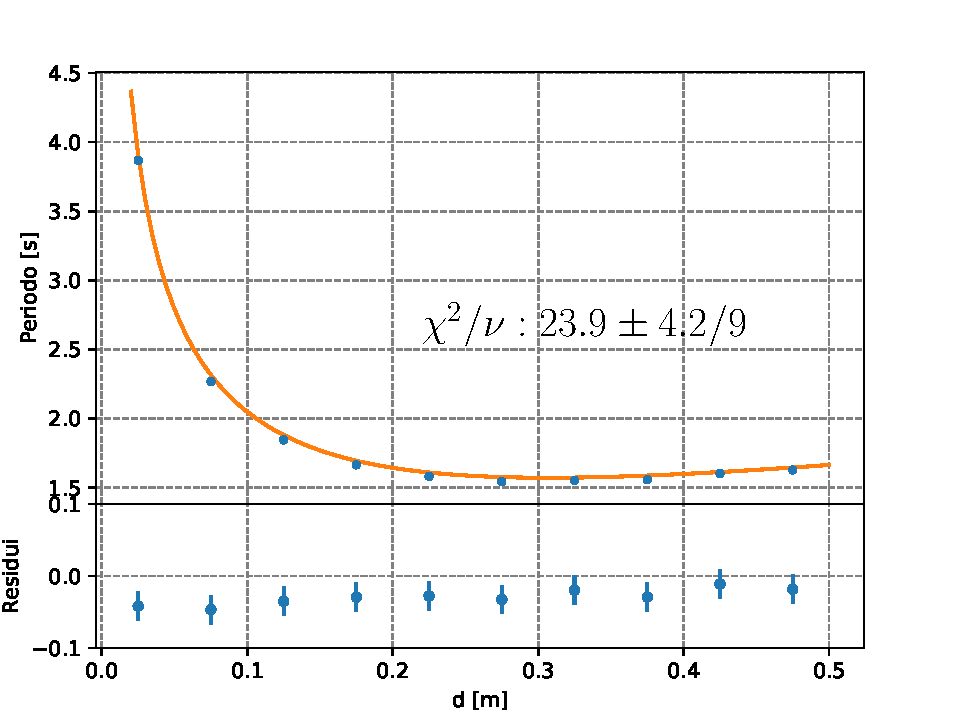
\includegraphics[width=0.8\textwidth]{extra/Periodo_lunghezza.pdf}
            \caption{Grafico dei periodi in funzione della distanza del centro di massa.}
            \label{fig:Periodo_lunghezza}
        \end{figure}
    

    
    \section{Conclusioni}
        Come si può chiaramente vedere dal grafico, i dati che sono stati riportati seguono approssimativamente un andamento iperbolico;
        il valore ottenuto per il $\chi^2$ è a circa $3.5$ sigma dal suo valore di aspettazione,
        quindi non possiamo escludere completamente la possibilità che il modello teorico
        sia adeguato.
        Tuttavia si nota che i valori dei residui risultano tutti negativi,
        questo potrebbe indicare la presenza di un errore sistematico,
        possibilmente causato dall'attrito (trascurato dal modello teorico) o dall'approssimazione $\sin \theta \sim \theta$.
        
\end{document}
